\documentclass[a4paper,12pt]{report}

% Regolazione margini
\usepackage{geometry}
\geometry{a4paper, top=1.9cm, bottom=2cm, left=2cm, right=2cm}

\usepackage{alltt, fancyvrb, url}
\usepackage{graphicx}
\usepackage[utf8]{inputenc}
\usepackage{hyperref}
\usepackage{float}

\usepackage[italian]{babel}

\usepackage[italian]{cleveref}

% Grafica e personalizzazione
\usepackage{graphicx}
\usepackage{booktabs}
\usepackage{keyval}
\usepackage{sidecap}
\usepackage{caption}
\usepackage{wrapfig}
\usepackage{floatflt}
\usepackage{imakeidx}
\usepackage{amssymb}
\usepackage{wasysym}
\usepackage[dvipsnames,usenames]{xcolor}
\usepackage{tikz}

% Colorare e modificare le tabelle
\usepackage{array}
\newcolumntype{L}[1]{>{\raggedright\arraybackslash}p{#1}}
\newcolumntype{C}[1]{>{\centering\arraybackslash}p{#1}}
\newcolumntype{R}[1]{>{\raggedleft\arraybackslash}p{#1}}
\usepackage{colortbl}
\usepackage{multirow}
%tabella senza linee 
\newcommand{\quantities}[1]{ %serve per inserire dati nella tabella   
	\begin{tabular}{@{}c@{}}\strut#1\strut\end{tabular}%
}

\title{\textbf{DB-Garage}\\Relazione per\\``Elaborato di Basi di Dati''}

\author{Barberini Elisa\\Mainardi Giosuè Giocondo}
\date{\today}

\begin{document}

\maketitle

\tableofcontents

\chapter{Analisi dei requisiti}
L'autofficina \textbf{DB-Garage}$^{\copyright}$ richiede la realizzazione di un database per la gestione di automobili,
%
clienti, dipendenti e delle loro interazioni, ovvero riparazioni e acquisto o vendita dei veicoli. Vengono di seguito 
%
descritti gli aspetti caratterizzanti del dominio.

\section{Intervista}

Di ogni utente del portale (cliente o impiegato) è necessario memorizzare: codice fiscale, nome, cognome,
%
data di nascita e telefono. Si può inoltre aggiungere, preferibilmente, anche una e-mail per le eventuali comunicazioni. 
%
I dipendenti si differenziano in base al tipo di attività che possono svolgere, che può essere quello di riparazioni o 
%
quello di compravendita.
%
Il primo tipo di lavoratori è formato da meccanici ed il secondo da agenti automobilistici, di entrambi si vuole memorizzare 
%
anche la retribuzione oraria.

Le automobili sono identificate da modello e casa produttrice, ma hanno anche cilindrata e anno di produzione.
%
Ciascun veicolo può essere oggetto di molteplici attestati di proprietà con il suo utente proprietario, 
%
ma un auto potrà avere solo un attestato non scaduto, altrimenti vorrà dire che è di proprietà dell'officina.

Ogni riparazione ad una determinata automobile coinvolge uno o più meccanici per ciascuno dei quali deve 
%
essere tenuta traccia del numero di ore dedicate.
%
Inoltre, il sistema deve considerare gli eventuali pezzi di ricambio utilizzati che sono individuati da 
%
casa produttrice e modello di riferimento, con l'aggiunta del costo unitario e una breve descrizione se necessaria.
%
Il costo totale di ciascuna riparazione viene stabilito a lavoro finito, basandosi sul conto delle ore 
%
impiegate di ciascun meccanico e dell’utilizzo di eventuali pezzi di ricambio.

Ogni transazione nel reparto compravendita viene effettuata da un agente automobilistico con un cliente 
%
e riguarda uno specifico veicolo, di essa si vogliono memorizzare se sia acquisto(l'officina compra l'auto 
%
dall'utente) o vendita(l'officina vende l'auto ad un utente), prezzo concordato e la data. 
% 
Una transazione, una volta effettuata, determinerà un passaggio di proprietà del veicolo in oggetto

La base di dati deve mantenere in memoria sia la data di inizio che la data di fine di ogni riparazione effettuata,
%
di ogni transazione e di ogni attestato di proprietà, così da poter essere mostrati in caso di richiesta dai clienti.

\section{Tabella concetti principali con sinonimi e definizioni}

\begin{figure}[H]
	\fontsize{10pt}{12pt}\selectfont
	\advance\leftskip-4cm
	\centering
	\arrayrulecolor{BlueGreen}
	\begin{tabular}{l c c }
		\rowcolor{BlueGreen}
		\rule[-3mm]{0mm}{0.85cm}
		\textbf{Termine} & \textbf{Eventuali sinonimi} &\textbf{Breve descrizione} \\
		\hline\rule[-3mm]{0mm}{0.85cm}
		Utente & & \quantities{Persona registrata nel sistema.} \\
		\hline\rule[-3mm]{0mm}{0.85cm}
		Dipendente & \quantities{Impiegato, Lavoratore} & \quantities{Persona che lavora per l'officina \\come meccanico o agente.} \\
		\hline\rule[-3mm]{0mm}{0.85cm}
		Cliente & & \quantities{Persona che deve eseguire o ha eseguito una \\riparazione o una transazione con l'officina. }\\
		\hline\rule[-3mm]{0mm}{0.85cm}
		Meccanico & & \quantities{Dipendente dell'officina che esegue riparazioni.} \\
		\hline\rule[-3mm]{0mm}{0.85cm}
		Agente & Agente automobilistico & \quantities{Dipendente dell'officina che esegue transazioni.}\\
		\hline\rule[-3mm]{0mm}{0.85cm}
		Riparazione & Lavoro & \quantities{Servizio di uno o più meccanici riguardo a un \\veicolo, su richiesta di un cliente.}\\
		\hline\rule[-3mm]{0mm}{0.85cm}
		Transazione & & \quantities{Servizio di un agente per l'acquisto o la \\vendita di un auto da parte di un cliente.}\\
		\hline\rule[-3mm]{0mm}{0.85cm}
		Veicolo & \quantities{Auto, \\ Automobile} & Oggetto dei servizi dell'officina.  \\
		\hline\rule[-3mm]{0mm}{0.85cm}
		Attestato & Attestato di proprietà & \quantities{Documento che certifica l'appartenenza di \\un auto ad una determinata persona.} \\
		\hline\rule[-3mm]{0mm}{0.85cm}
		Acquisto &  & \quantities{Transazione che determina il passaggio di \\proprietà di un auto da un cliente all'officina.} \\
		\hline\rule[-3mm]{0mm}{0.85cm}
		Vendita &  & \quantities{Transazione che determina il passaggio di \\proprietà di un auto dall'officina ad un cliente.} \\
		\hline\rule[-3mm]{0mm}{0.85cm}
		Pezzo di ricambio &  & \quantities{Articolo che può essere necessario \\per la riparazione di un auto.} \\
		\hline
	\end{tabular}
\end{figure}
\section{Definizione specifiche in linguaggio naturale}
L'autofficina \textbf{DB-Garage}$^{\copyright}$ richiede la realizzazione di un database per la gestione di automobili,
%
clienti, dipendenti e delle loro interazioni, ovvero riparazioni e acquisto o vendita dei veicoli. Vengono di seguito 
%
descritti gli aspetti caratterizzanti del dominio.

Un \textbf{Utente} è una persona registrata nel sistema della quale è necessario memorizzare: codice fiscale, nome, cognome,
%
data di nascita e telefono, più una e-mail opzionale.

Un \textbf{Cliente} è una semplice sottoclasse di Utente senza attributi aggiuntivi, che ha effettuato o deve effettuare 
%
una Riparazione o una Transazione.

\textbf{Dipendente} è un'altra sottoclasse ma che ha anche una paga oraria e due sottoclassi a sua volta: \textbf{Meccanico} e \textbf{Agente}.

L'oggetto principale delle operazioni del sistema è il \textbf{Veicolo} che è identificato da modello e casa produttrice, ma ha anche cilindrata e anno di produzione.
%
Ciascun Veicolo può essere oggetto di molteplici \textbf{Attestati} con il suo \underline{Utente proprietario}, 
%
ma un Veicolo potrà avere solo un Attestato non scaduto, altrimenti vorrà dire che è di proprietà dell'\textit{Officina}.

Ogni \textbf{Riparazione} ad un determinato Veicolo coinvolge uno o più \textbf{Meccanici} per ciascuno dei quali deve 
%
essere tenuta traccia del numero di ore dedicate.

Inoltre, il sistema deve considerare gli eventuali \textbf{Pezzi di ricambio} utilizzati che sono individuati da 
%
casa produttrice e modello di riferimento, con l'aggiunta del costo unitario e una breve descrizione, opzionale.

Il costo totale di ciascuna Riparazione viene stabilito all'inserimento nel sistema, tenendo conto delle ore 
%
impiegate da ciascun Meccanico e della quantità dei Pezzi di ricambio.

Ogni \textbf{Transazione} viene effettuata da un \textbf{Agente} con un \textbf{Cliente} e riguarda un specifico \textbf{Veicolo},
%
di essa si vuole memorizzare se sia acquisto(l'\textit{Officina} compra l'auto dall'Utente) o vendita(l'\textit{Officina} 
% 
vende l'auto ad un Utente), prezzo e data. 

Una Transazione determina un passaggio di proprietà del Veicolo in oggetto, quindi il relativo \textbf{Attestato} 
%
dovrà essere posto come scaduto e ne sarà inserito un altro se il Veicolo passa ad un Cliente(\underline{Transazione di Vendita}),
%
mentre se passa all'\textit{Officina}(\underline{Transazione di Acquisto}) no.

Devono essere tenute in memoria sia la data di inizio che la data di fine di ogni Riparazione effettuata, di ogni Transazione e di 
%
ogni Attestato.

\subsection*{Principali azioni richieste:}
\begin{enumerate}
	\item Inserimento nuovo cliente
	\item Inserimento nuovo veicolo
	\item Inserimento riparazione
	\item Inserimento transazione
	\item Inserimento atto di proprietà
	\item Visualizza elenco clienti
	\item Visualizza elenco meccanici
	\item Visualizza elenco agenti
	\item Visualizza elenco riparazioni effettuate da un meccanico
	\item Visualizza elenco pezzi ricambi usati per una certa riparazione
	\item Visualizza elenco veicoli che possiede un determinato cliente
	\item Visualizza elenco solo veicoli in vendita (veicoli dell'officina)
	\item Aggiorna attributo scaduto su atto di proprietà
\end{enumerate}

\chapter{Progettazione Concettuale}

\section{Schema Scheletro}

\section{Raffinamenti}

\section{Schema Finale}
\addcontentsline{toc}{section}{Schema Finale}	
	\begin{figure}[h!]
		\centering
		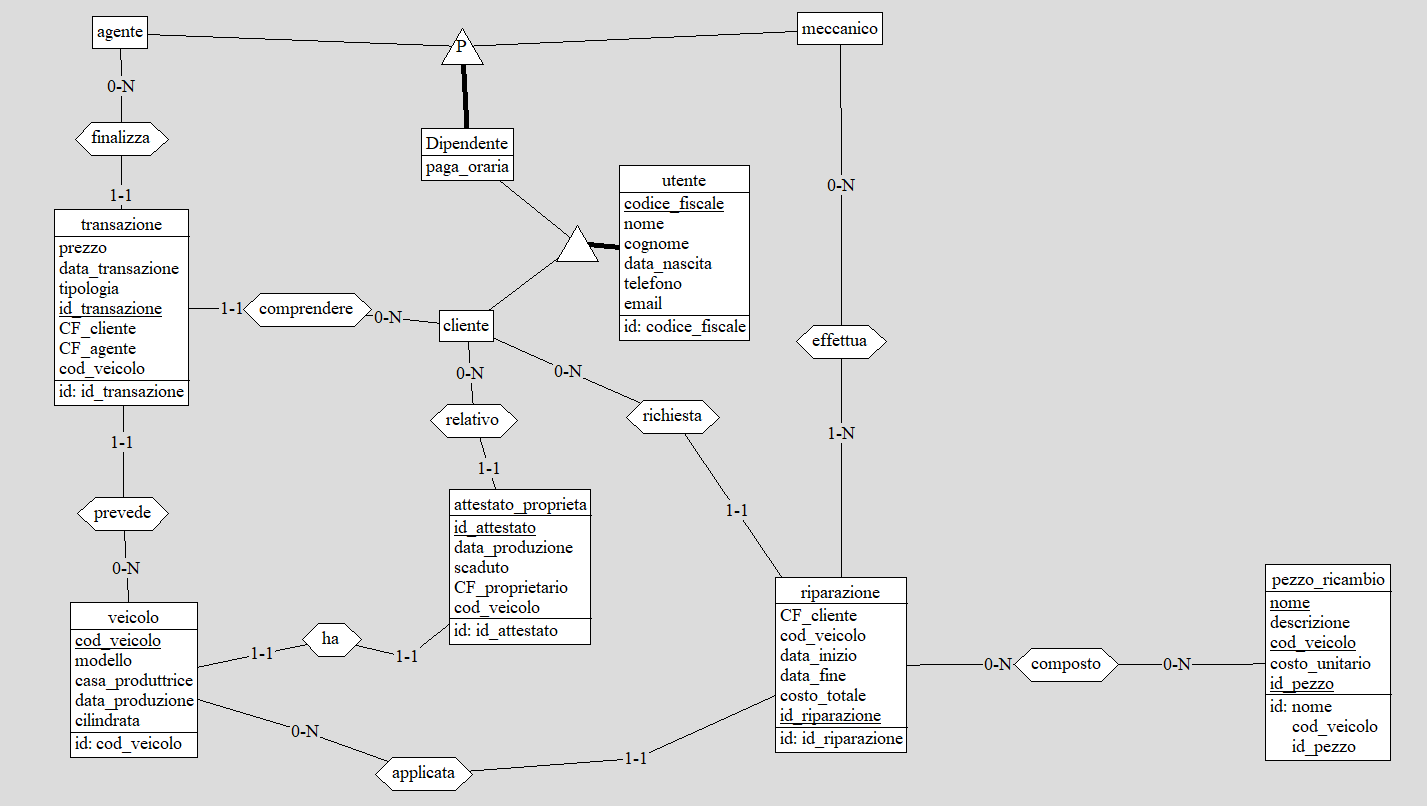
\includegraphics[scale=0.56]{img/schema_finale.png}
	\end{figure}

\chapter{Progettazione Logica}

\section{Stima Volume dati}
\begin{figure}[H]
	\fontsize{14pt}{12pt}\selectfont
	\advance\leftskip-15cm
	\centering
	\arrayrulecolor{BlueGreen}
	\begin{tabular}{l c c }
		\rowcolor{BlueGreen}
		\rule[-3mm]{0mm}{0.85cm}
		\textbf{Concetto} & \textbf{Costrutto} &\textbf{Volume} \\
		\hline\rule[-2mm]{0mm}{0.75cm}
		Utente & E & 3050\\
		\hline\rule[-2mm]{0mm}{0.75cm}
		Cliente & E & 3000 \\
		\hline\rule[-2mm]{0mm}{0.75cm}
		Dipendente & E & 50\\
		\hline\rule[-2mm]{0mm}{0.75cm}
		Agente & E & 20\\
		\hline\rule[-2mm]{0mm}{0.75cm}
		Meccanico & E & 30\\
		\hline\rule[-2mm]{0mm}{0.75cm}
		Possesso & R & 6000 \\
		\hline\rule[-2mm]{0mm}{0.75cm}
		Attestato & R & 6000\\
		\hline\rule[-2mm]{0mm}{0.75cm}
		Riguardo & R & 6000 \\
		\hline\rule[-2mm]{0mm}{0.75cm}
		Veicolo & E & 5000 \\
		\hline\rule[-2mm]{0mm}{0.75cm}
		Coinvolgimento & R & 1000\\
		\hline\rule[-2mm]{0mm}{0.75cm}
		Transazione & R & 1000\\
		\hline\rule[-2mm]{0mm}{0.75cm}
		Transazione d'acquisto& R & 400\\
		\hline\rule[-2mm]{0mm}{0.75cm}
		Transazione di vendita& R & 600\\
		\hline\rule[-2mm]{0mm}{0.75cm}
		Perseguimento & R & 1000\\
		\hline\rule[-2mm]{0mm}{0.75cm}
		Esecuzione & R & 1000\\
		\hline\rule[-2mm]{0mm}{0.75cm}
		Lavorazione & R & 12000\\
		\hline\rule[-2mm]{0mm}{0.75cm}
		Riparazione & E & 12000\\
		\hline\rule[-2mm]{0mm}{0.75cm}
		Richiesta & R & 12000\\
		\hline\rule[-2mm]{0mm}{0.75cm}
		Sottoposizione & R & 12000\\
		\hline\rule[-2mm]{0mm}{0.75cm}
		Utilizzo & R & 15000\\
		\hline\rule[-2mm]{0mm}{0.75cm}
		Pezzo di ricambio & E &  9000\\
		\hline
	\end{tabular}
\end{figure}

\section{Descrizione operazioni principali e stima frequenza}
\begin{figure}[H]
	\fontsize{14pt}{12pt}\selectfont
	\advance\leftskip-15cm
	\centering
	\arrayrulecolor{BlueGreen}
	\begin{tabular}{c c c }
		\rowcolor{BlueGreen}
		\rule[-6mm]{0mm}{1.5cm}
		\textbf{Codice} & \textbf{Operazione} &\textbf{Frequenza} \\
		\hline\rule[-5mm]{0mm}{1.4cm}
		1 & Inserimento nuovo cliente & 5 al giorno \\
		\hline\rule[-5mm]{0mm}{1.4cm}
		2 & Inserimento nuovo veicolo & 6 al giorno \\
		\hline\rule[-5mm]{0mm}{1.4cm}
		3 & Inserimento riparazione & 20 al giorno \\
		\hline\rule[-5mm]{0mm}{1.4cm}
		4 & Inserimento transazione & 2 a settimana \\
		\hline\rule[-5mm]{0mm}{1.4cm}
		5 & Inserimento atto di proprietà & 4 a settimana \\
		\hline\rule[-5mm]{0mm}{1.4cm}
		6 & Visualizza elenco clienti & 25 al giorno \\
		\hline\rule[-5mm]{0mm}{1.4cm}
		7 & Visualizza elenco meccanici & 22 al giorno \\
		\hline\rule[-5mm]{0mm}{1.4cm}
		8 & Visualizza elenco agenti & 3 a settimana \\
		\hline\rule[-5mm]{0mm}{1.4cm}
		9 & \quantities{Visualizza elenco riparazioni\\effettuate da un meccanico} & 1 al giorno \\
		\hline\rule[-5mm]{0mm}{1.4cm}
		10 & \quantities{Visualizza elenco pezzi ricambi\\usati per una certa riparazione} & 1 al giorno \\
		\hline\rule[-5mm]{0mm}{1.4cm}
		11 & \quantities{Visualizza elenco veicoli che\\possiede un determinato cliente} & 22 al giorno \\
		\hline\rule[-5mm]{0mm}{1.4cm}
		12 & \quantities{Visualizza elenco solo\\veicoli in vendita} & 3 al giorno\\
		\hline\rule[-5mm]{0mm}{1.4cm}
		13 & \quantities{Aggiorna attributo scaduto\\su atto di proprietà} & 2 a settimana \\
		\hline
	\end{tabular}
\end{figure}
\newpage
\section{Schemi di navigazione e tabelle accessi}
\subsection*{Operazione 1: Inserimento cliente}
\begin{figure}[ht]
	\centering
	\arrayrulecolor{BlueGreen}
	\begin{tabular}{L{3cm}C{2.5cm}C{4.5cm}C{2.5cm}}
		\rowcolor{BlueGreen}\rule[-2mm]{0mm}{0.65cm}{}
		\textbf{Concetto} & \textbf{Costrutto} &\textbf{Accessi} & \textbf{Tipo} \\	
		\hline\rule[-2mm]{0mm}{0.65cm}{}
		Cliente & E & 1 & S \\
	\end{tabular}
	
	\begin{tabular}{C{13.9cm}}
		\rule[-2.5mm]{0mm}{0.8cm}{}	
		\cellcolor{BlueGreen} \textbf{\underline{Totale:} 1 S $\to$ 2 x 5 = 10 accessi al giorno}
	\end{tabular}
\end{figure}

\subsection*{Operazione 2: Inserimento veicolo}
\begin{figure}[ht]
	\centering
	\arrayrulecolor{BlueGreen}
	\begin{tabular}{L{3cm}C{2.5cm}C{4.5cm}C{2.5cm}}
		\rowcolor{BlueGreen}\rule[-2mm]{0mm}{0.65cm}{}
		\textbf{Concetto} & \textbf{Costrutto} &\textbf{Accessi} & \textbf{Tipo} \\
		\hline\rule[-2mm]{0mm}{0.65cm}{}
		Cliente & E & 3 000 & L \\
		\hline\rule[-2mm]{0mm}{0.65cm}{}
		Veicolo & E & 1 & S \\
	\end{tabular}
	
	\begin{tabular}{C{13.9cm}}
		\rule[-2.5mm]{0mm}{0.8cm}{}	
		\cellcolor{BlueGreen} \textbf{\underline{Totale:} 1 S + 3 000 L $\to$ 3 002 x 6 = 18 012 accessi al giorno}
	\end{tabular}
\end{figure}

\subsection*{Operazione 3: Inserimento riparazione}
\begin{figure}[ht]
	\centering
	\arrayrulecolor{BlueGreen}
	\begin{tabular}{L{3cm}C{2.5cm}C{4.5cm}C{2.5cm}}
		\rowcolor{BlueGreen}\rule[-2mm]{0mm}{0.65cm}{}
		\textbf{Concetto} & \textbf{Costrutto} &\textbf{Accessi} & \textbf{Tipo} \\

	\end{tabular}
	
	\begin{tabular}{C{13.9cm}}
		\rule[-2.5mm]{0mm}{0.8cm}{}	
		\cellcolor{BlueGreen} \textbf{\underline{Totale:} S + L $\to$  accessi al giorno}
	\end{tabular}
\end{figure}

\section{Raffinamento schema}
...eliminazione di identificatori esterni, attributi composti e gerarchie, scelta delle chiavi

\section{Analisi ridondanze}

\section{Traduzione di entità e associazioni in relazioni}

\section{Schema relazionale finale}

\section{Traduzione delle operazioni in query SQL}

\chapter{Progettazione Applicazione}

\section{Descrizione applicazione}

DA INSERIRE: Screenshot interfaccia utente

\end{document}
